\chapter{Architektur}
Die folgenden UML-Diagramme sind nicht vollständig.
Wir versuchen einen kleinen aber dennoch guten Einblick in unsere Architektur zu liefern.
Dieser Abschnitt sicher spannend für technikinteressierte Leser. Man muss jedoch kein Informatiker sein, um dieses Kapitel zu verstehen.

\section{Klassendiagramm}
Folgend ist der Klassenaufbau unseres Spieles zu sehen.
Das rote (S) steht für Singleton.
Dies sind Klassen, die im ganzen Spiel nur genau einmal existieren können.
Die erste Graphik zeigt den momentanen Stand, wobei mit der Entwicklung des Deckbauers die neue Klasse "DeckManager" hinzukommen wird. 
\begin{figure}[H]
    \centering
    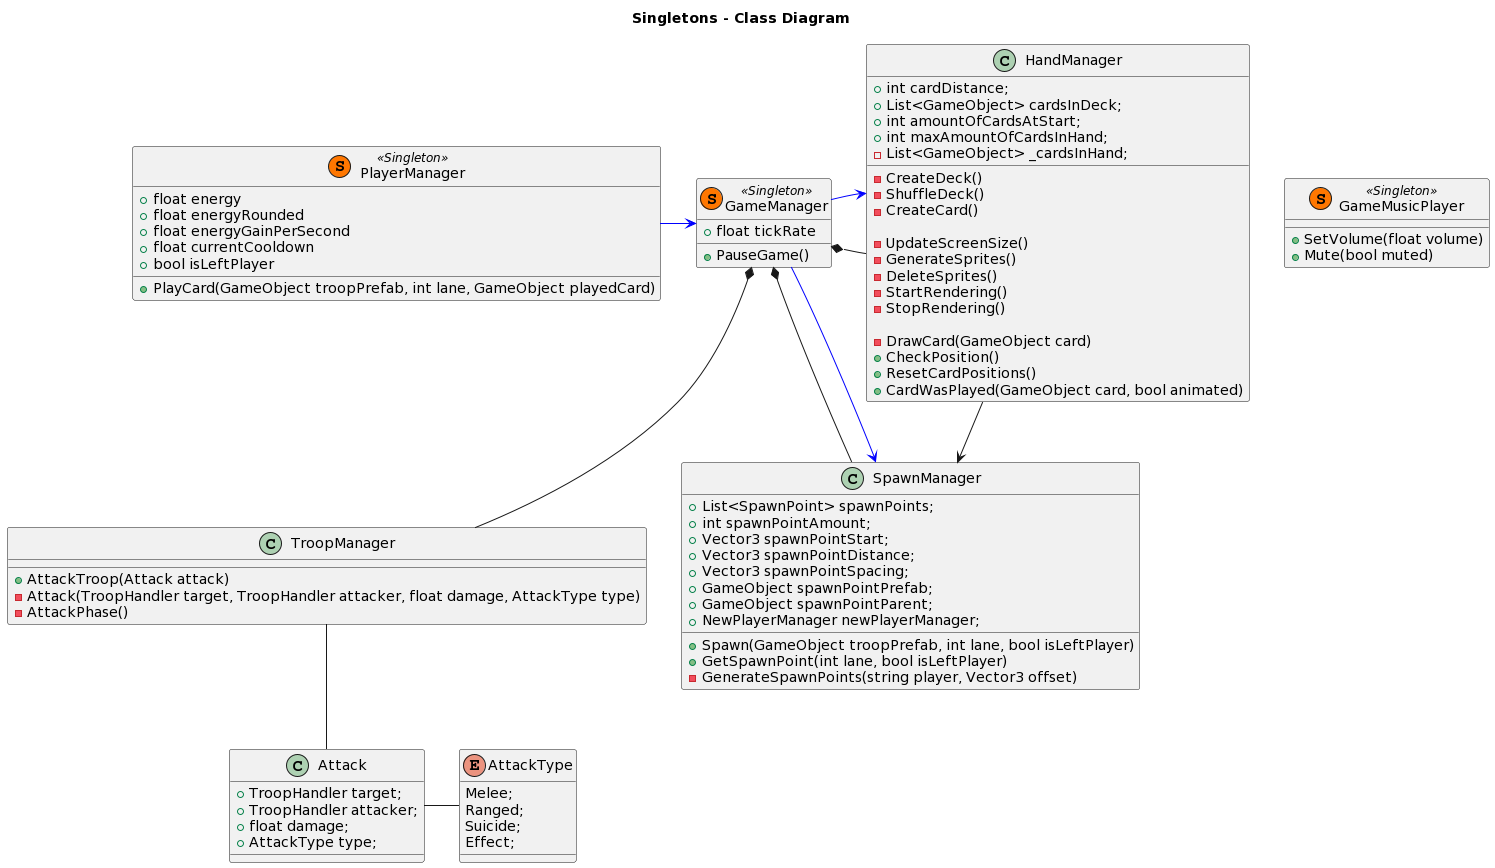
\includegraphics[width=13cm]{resources/Singletons.png} \\
    \caption{momentaner Aufbau}
\end{figure}

\begin{figure}[H]
    \centering
    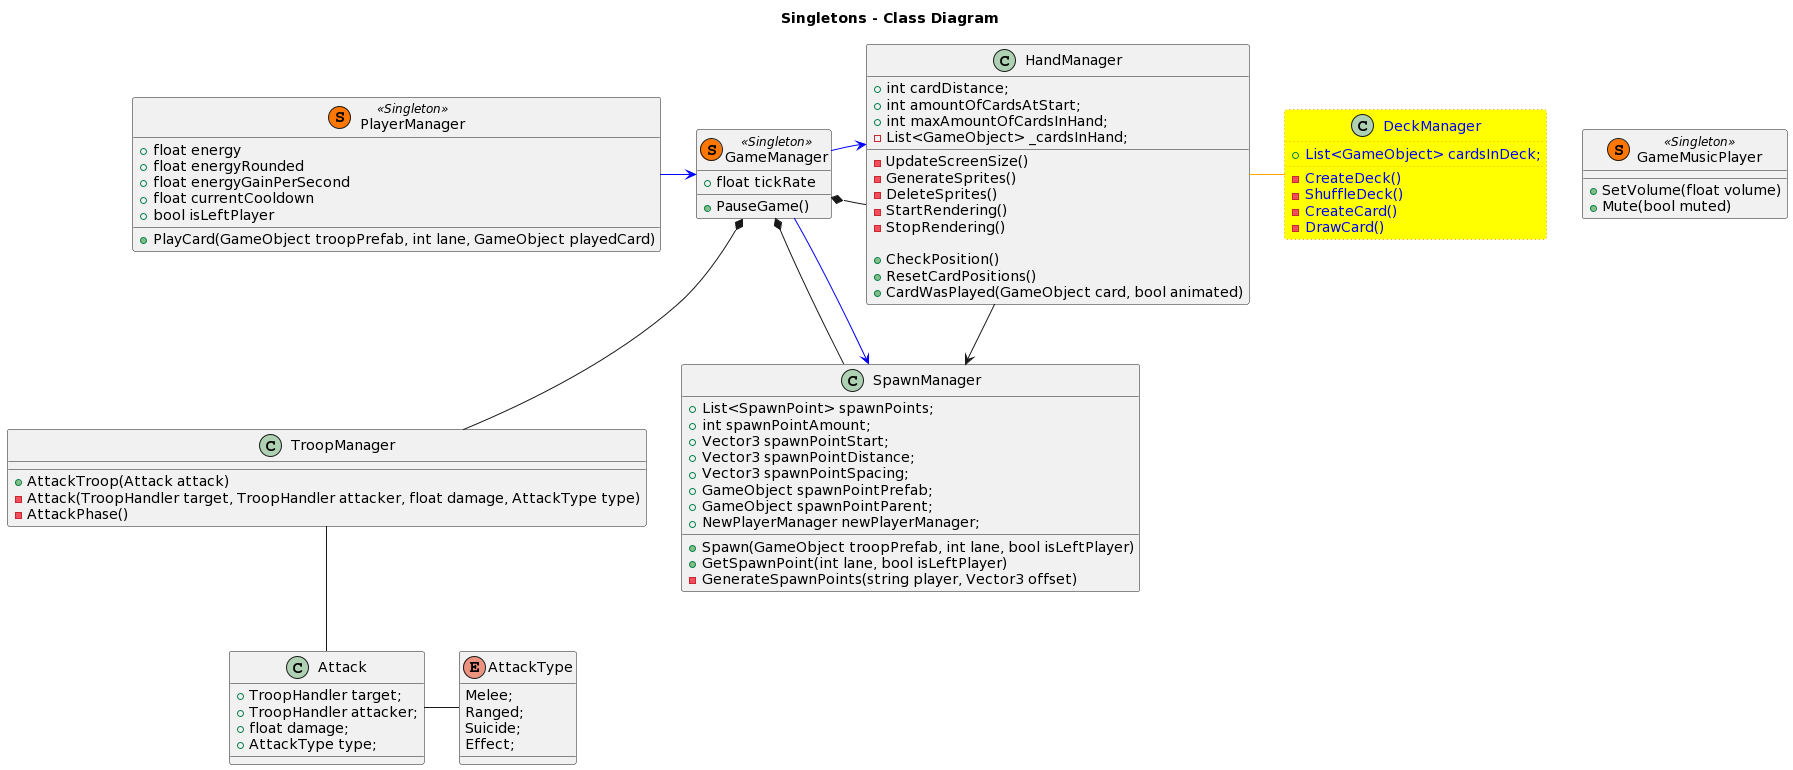
\includegraphics[width=13cm]{resources/Singletons 2.png} \\
    \caption{zukünftiger Aufbau}
\end{figure}

\section{Sequenzdiagramme}
\subsection{Nahkampftruppe}
\begin{figure}[H]
    \centering
    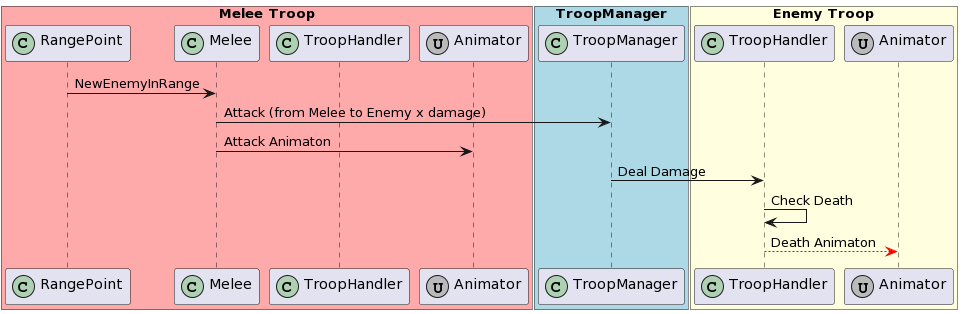
\includegraphics[width=15cm]{resources/MeleeAttacks.png}\\
    \caption{Abfolge, wenn eine Truppe in Reichweite einer Nahkampftruppe kommt}
\end{figure}

\subsection{Suizidtruppe}
\begin{figure}[H]
    \centering
    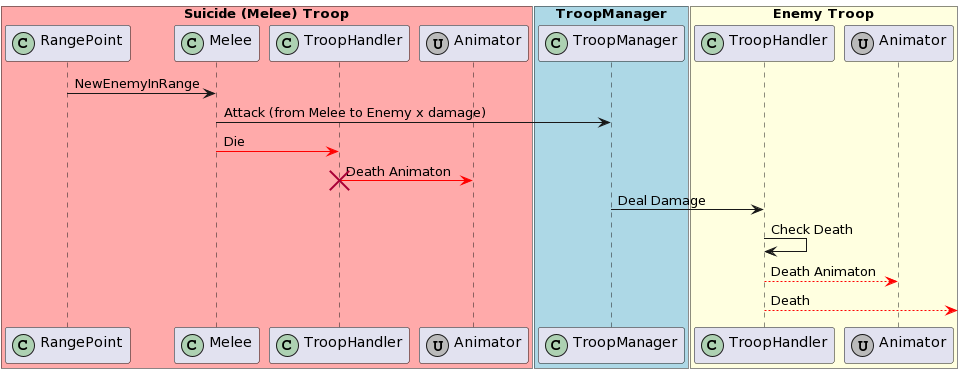
\includegraphics[width=15cm]{resources/SuicideAttacks.png}\\
    \caption{Suizidtruppe mit ähnlichen Prinzipien}
\end{figure}



\subsection{Fernkampftruppe}
\begin{figure}[H]
    \centering
    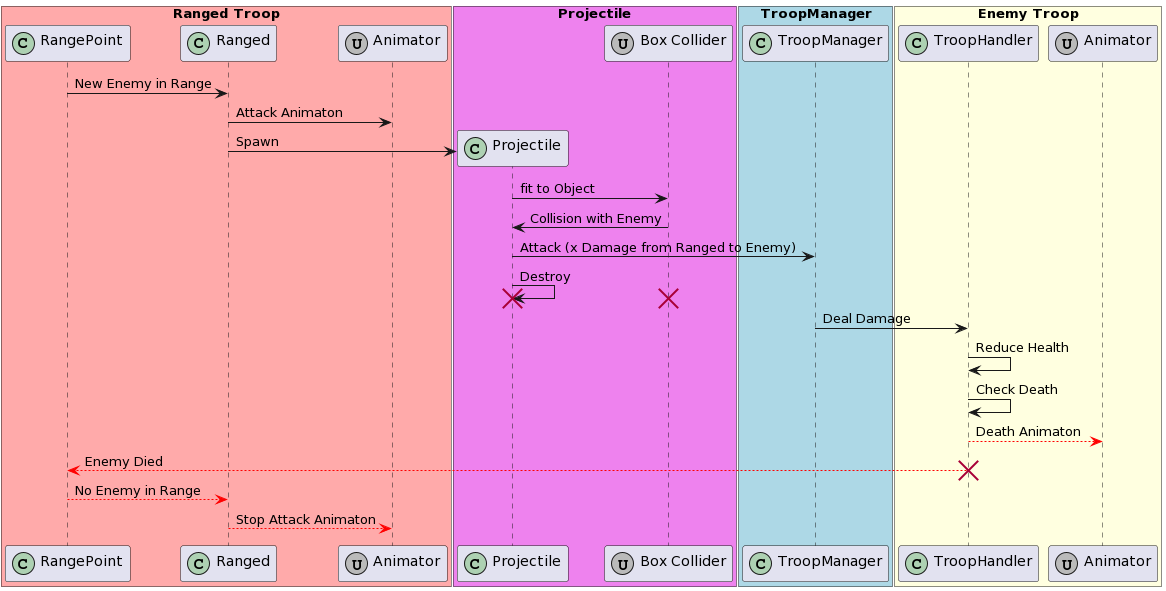
\includegraphics[width=15cm]{resources/RangedAttacks.png}\\
    \caption{Reaktion einer Fernkampftruppe auf neuen Gegner}
\end{figure}
\begin{figure}[H]
    \centering
    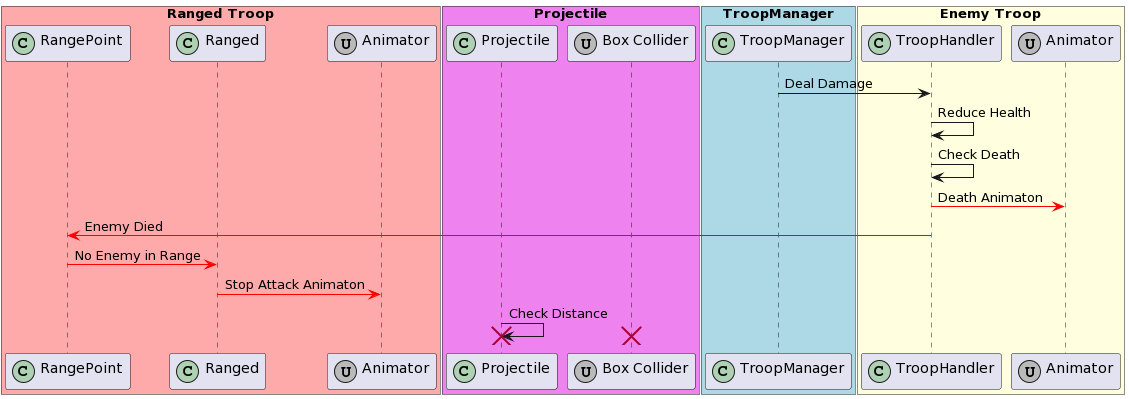
\includegraphics[width=15cm]{resources/Projectile.png}\\
    \caption{Gegner stirbt bevor das Projektil Schaden anrichten konnte}
\end{figure}


\subsection{Gift}
\begin{figure}[H]
    \centering
    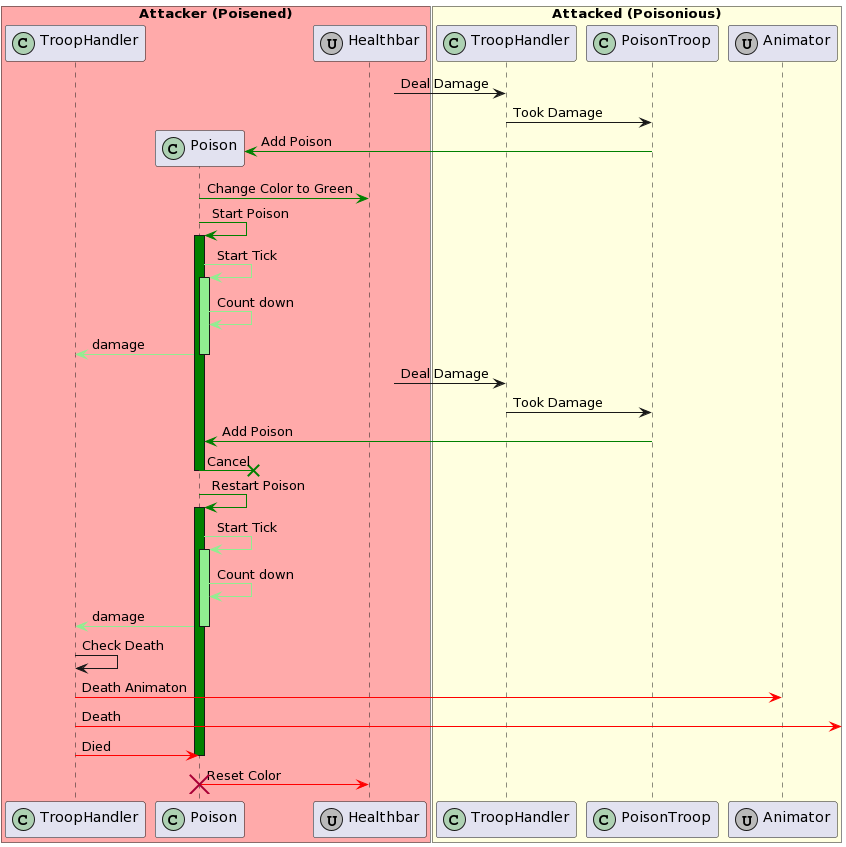
\includegraphics[width=15cm]{resources/Poison.png} \\
    \caption{Reaktion einer Truppe die den Effekt Gift besitzt}
\end{figure}


\section{GitHub source control}
Die Visualisierung von unserem GitHub Repository kann man unter folgendem Link \url{https://youtu.be/3uPTdjVXtNk} einsehen.